\documentclass[letterpaper,12pt,fleqn]{article}
\usepackage{matharticle}
\usepackage{siunitx}
\pagestyle{plain}
\renewcommand{\o}{\theta}
\newcommand{\p}{\phi}
\begin{document}

\begin{center}
\Large Math-19 Homework \#16 Solutions
\end{center}

\vspace{0.5in}

\underline{Problems}

\begin{enumerate}
\item Prove that the following is an identity:
  \[\frac{1}{\csc{x}+\cot{x}}+\frac{1}{\csc{x}-\cot{x}}=2\csc{x}\]

  \begin{eqnarray*}
    \frac{1}{\csc{x}+\cot{x}}+\frac{1}{\csc{x}-\cot{x}} &=&
    \frac{(\csc{x}-\cot{x})+(\csc{x}+\cot{x})}{\csc^2x-\cot^2x} \\
    &=& \frac{2\csc{x}}{1} \\
    &=& 2\csc{x} \\
  \end{eqnarray*}

\item: Write the following as a function of $x$ with no trig functions:
  \[\sin\left(\sec^{-1}\frac{1}{\sqrt{1-x^2}}+\csc^{-1}\sqrt{1+x^2}\right)\]

  Let:
  \[\o_1=\sec^{-1}\frac{1}{\sqrt{1-x^2}}\]
  \[\o_2=\csc^{-1}\sqrt{1+x^2}\]

  \begin{minipage}{3in}
    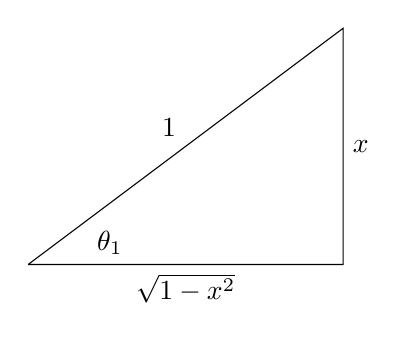
\begin{tikzpicture}
      \draw (0,0) -- (4,0) -- (4,3) -- (0,0);
      \node [below] at (2,0) {$\sqrt{1-x^2}$};
      \node [right] at (4,1.5) {$x$};
      \node [above left] at (2,1.5) {$1$};
      \node [above right] at (0.75,0) {$\o_1$};
    \end{tikzpicture}
  \end{minipage}
  \begin{minipage}{3in}
    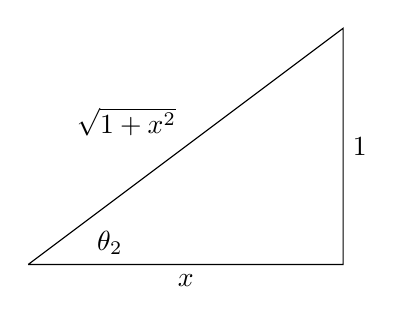
\begin{tikzpicture}
      \draw (0,0) -- (4,0) -- (4,3) -- (0,0);
      \node [below] at (2,0) {$x$};
      \node [right] at (4,1.5) {$1$};
      \node [above left] at (2,1.5) {$\sqrt{1+x^2}$};
      \node [above right] at (0.75,0) {$\o_2$};
    \end{tikzpicture}
  \end{minipage}

  \begin{eqnarray*}
    \sin(\o_1+\o_2) &=& \sin\o_1\cos\o_2+\cos\o_1\sin\o_2 \\
    &=& \left(\frac{x}{1}\right)\left(\frac{x}{\sqrt{1+x^2}}\right)+
    \left(\frac{\sqrt{1-x^2}}{1}\right)\left(\frac{1}{\sqrt{1+x^2}}\right) \\
    &=& \frac{x^2+\sqrt{1-x^2}}{\sqrt{1+x^2}} \\
  \end{eqnarray*}

\item Write the following as a single sine function. Note that you can use
  approximate value (i.e., your calculator) for the various coefficient and
  angle calculation. Use 4 decimal places.
  \[\cos\left(x+\frac{\pi}{3}\right)+\sin\left(x-\frac{\pi}{4}\right)\]

  First, use the sum and difference formulas in order to get simple sine and
  cosine terms:

  \begin{eqnarray*}
    \cos\left(x+\frac{\pi}{3}\right)+\sin\left(x-\frac{\pi}{4}\right) &=&
    \left(\cos{x}\cos{\frac{\pi}{3}}-\sin{x}\sin{\frac{\pi}{3}}\right)+
    \left(\sin{x}\cos{\frac{\pi}{4}}-\cos{x}\sin{\frac{\pi}{4}}\right) \\
    &=& \frac{1}{2}\cos{x}-\frac{\sqrt{3}}{2}\sin{x}+
    \frac{1}{\sqrt{2}}\sin{x}-\frac{1}{\sqrt{2}}\cos{x} \\
    &=& \left(\frac{1}{\sqrt{2}}-\frac{\sqrt{3}}{2}\right)\sin{x}+
    \left(\frac{1}{2}-\frac{1}{\sqrt{2}}\right)\cos{x} \\
    &=& -0.1589\sin{x}-0.2071\cos{x} \\
  \end{eqnarray*}

  Next, calculate the new amplitude:

  $A=\sqrt{(-0.1589)^2+(-0.2071)^2}=0.2610$

  and then divide it out:

  $A\left(\frac{-0.1589}{A}\sin{x}+\frac{-0.2071}{A}\cos{x}\right)$

  We want a single sine function of the form:

  $A\sin(x+\p)=A(\sin x\cos\p+\cos x\sin\p)$

  And so:

  $\cos\p=\frac{-0.1589}{A}$\qquad$\sin\p=\frac{-0.2071}{A}$

  And thus:

  $\tan\p=\frac{\sin\p}{\cos\p}=\frac{-0.2071}{-0.1589}$

  Next, draw a triangle for $\p$ in the proper quadrant. Note that since the
  horizontal ($\cos$) and vertical ($\sin$) sides are negative, $\p$ will be
  in QIII:

  \begin{center}
    \begin{tikzpicture}
      \draw (-5,0) -- (5,0);
      \draw (0,-5) -- (0,5);
      \draw [line width=1mm] (0,0) to node [above]  {$-0.1589$} (-2,0);
      \draw [line width=1mm] (-2,0) to node [left] {$-0.2071$} (-2,-4);
      \draw [dashed] (0,0) -- node [below] {$A$} (-2,-4);
      \node at (-0.5,-0.25) {$\p$};
    \end{tikzpicture}
  \end{center}

  Now calculate $\p$ using $\tan^{-1}$ on your calculator. Be careful! Your
  calculator is going to give you the angle in the reduced domain, in this
  case QI; however, the actual angle is in QIII. So, you must add $\pi$ to the
  value you get from your calculator to get the correct angle in QIII:

  $\p=tan^{-1}\frac{-0.2071}{-0.1589}+\pi\approx4.0579\approx232.5^{\circ}$

  Finally, putting it all together we get:

  $\cos\left(x+\frac{\pi}{3}\right)+\sin\left(x-\frac{\pi}{4}\right)=
  0.2610\sin(x+4.0579)=0.2610\sin(x+232.5^{\circ})$

  Generally, we prefer that $\p\in(-\pi,\pi]$, so subtract $2\pi$:

  $\cos\left(x+\frac{\pi}{3}\right)+\sin\left(x-\frac{\pi}{4}\right)=
  0.2610\sin(x-2.2253)=0.2610\sin(x-127.5^{\circ})$

\item Find \emph{all} possible solutions for $x$:
  \[2\sin^2x+(\sqrt{3}-4)\sin{x}-2\sqrt{3}=0\]
  $(2\sin{x}+\sqrt{3})(\sin{x}-2)=0$

  $\sin{x}=2$ has no solutions

  $\sin{x}=-\frac{\sqrt{3}}{2}$

  This occurs in QIII and QIV with a reference angle of $\frac{\pi}{3}$
  
  $x=-\frac{\pi}{3}+2\pi k$\qquad or\qquad$x=-\frac{2\pi}{3}+2\pi k$

\item Find \emph{all} possible solutions for $x$:
  \[\sin{2x}+\cos{x}=0\]

  $\sin2x+\cos x=2\sin x\cos x+\cos x=(2\sin x+1)\cos x=0$

  $\cos{x}=0$\qquad or\qquad$\sin{x}=-\frac{1}{2}$

  $x=\frac{\pi}{2}+\pi k$

  or
  
  $x=-\frac{\pi}{6}+2\pi k$\qquad or\qquad$x=-\frac{5\pi}{6}+2\pi k$
\end{enumerate}
 
\end{document}
